\section{3286 --- Find a Safe Walk Through a Grid (LeetCode)}

\subsection*{Código}
\lstinputlisting{3286_FindSafeWalk.java}

\subsection*{Comprovante de aceite}
\begin{center}
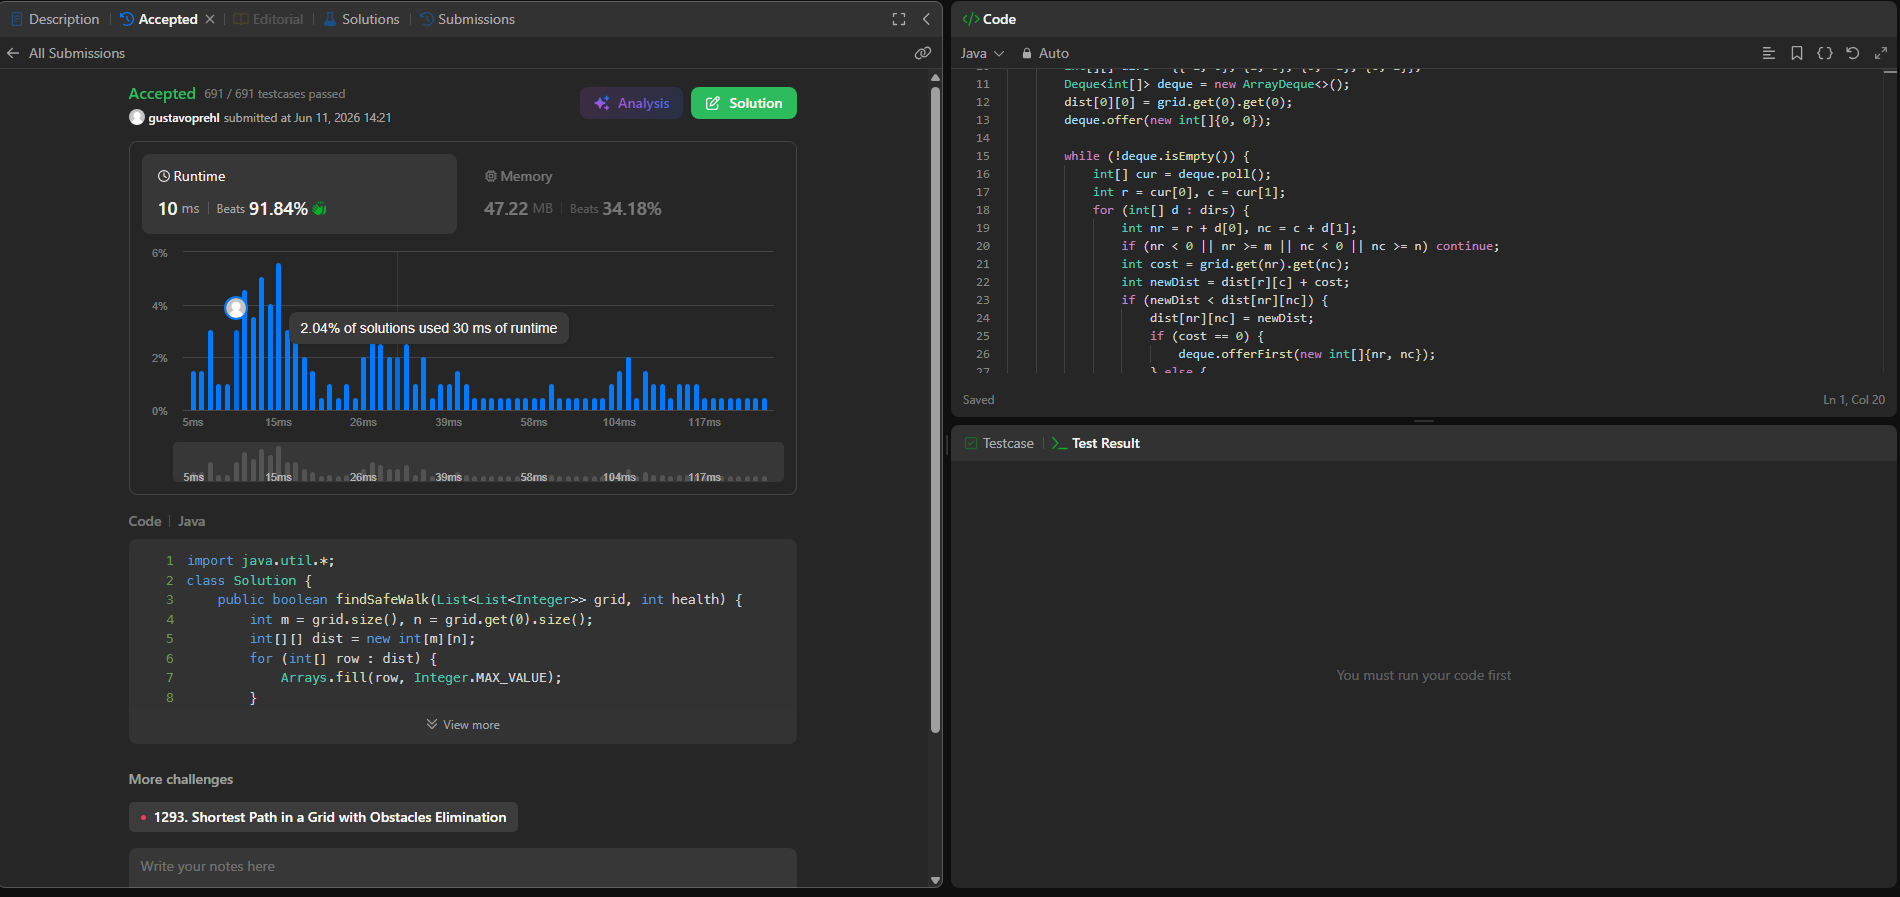
\includegraphics[width=0.85\textwidth]{Accepts/3286_FindSafeWalk_Submit.png}\\
\end{center}

\subsection*{Justificativa}

\textbf{Estratégia:} caminho mínimo em grafo com pesos $\{0, 1\}$ ---
algoritmo \textbf{0-1 BFS}, uma especialização do algoritmo de Dijkstra.

\textbf{Modelagem:} cada célula da grade é um vértice; há uma aresta entre
células adjacentes (4 direções). O ``custo'' de entrar em uma célula
\texttt{grid[i][j] = 1} é 1 (perde-se 1 ponto de vida) e o custo de uma
célula \texttt{grid[i][j] = 0} é 0. Definimos \texttt{dist[i][j]} como o
menor número total de células inseguras percorridas (incluindo a célula de
partida) em qualquer caminho de $(0,0)$ até $(i,j)$. A resposta é
\texttt{true} se e somente se \texttt{dist[m-1][n-1] <= health - 1}, ou seja,
se a vida restante ao chegar no destino for pelo menos 1.

\textbf{Por que o 0-1 BFS é correto (relação com Dijkstra):} o algoritmo de
Dijkstra processa vértices em ordem não decrescente de distância, garantindo
que, quando um vértice é retirado da estrutura, sua distância já é a
definitiva (propriedade da escolha gulosa + relaxamento de arestas). Como
aqui os pesos das arestas são apenas 0 ou 1, um deque substitui a fila de
prioridade: ao relaxar uma aresta de peso 0, o vizinho é inserido no início
do deque (mesma ``camada'' de distância); ao relaxar uma aresta de peso 1, o
vizinho é inserido no final (próxima camada). Essa invariante mantém o deque
sempre ordenado por distância, preservando a propriedade de Dijkstra sem
necessidade de heap.

\textbf{Complexidade:}
\begin{itemize}
    \item Tempo: $O(m \cdot n)$, pois cada célula é inserida/relaxada um
    número constante de vezes (grau $\leq 4$).
    \item Espaço: $O(m \cdot n)$ para a matriz \texttt{dist} e o deque.
\end{itemize}

\textbf{Tópico do curso:} a escolha gulosa de sempre expandir primeiro o
vértice de menor distância provisória (garantida pela ordenação do deque no
0-1 BFS) é a mesma propriedade de corretude do algoritmo de Dijkstra ---
\emph{Estratégia Gulosa e Divisão e Conquista} [CLRS09, caps. 4 e 16].
